\chapter{提案手法}
\label{chap:proposal}
本章では,生成クエリネットワークのメタ学習としての解釈に関する前章での議論を踏まえて,改善手法の提案を行う.前章で述べた通り,既存手法である生成クエリネットワークはシーン固有の知識をもつ変数$\bm{r_i}$をコンテキスト$D_i$から決定論的に推論しているため,コンテキストから推論可能なシーン表現の不確実性を考慮できていない.また,個別のデータに固有の潜在変数$\bm{z_i^k}$と,その事後分布$p(\bm{z_i^q}|\bm{x_i^q}, \bm{v_i^q}, \bm{r_i}; \theta)$を近似する$q(\bm{z_i^q}|\bm{x_i^q}, \bm{v_i^q}, \bm{r_i}; \phi)$の存在により,最適化すべきパラメータが増大してしまっているという問題点がある.そこで,提案手法では,生成クエリネットワークにおけるシーン表現$\bm{r_i}$と潜在変数$\bm{z_i^k}$を統合して,1つの確率的な潜在変数$\bm{z_i}$とすることで,モデルの冗長性を排除し,シーン表現の確率的な推論を可能にすることを目指す.

はじめに,提案手法で扱う問題設定について整理し,その後提案手法の具体的な説明として,確率モデル・最適化とモデルアーキテクチャについて述べていく.
%データの生成過程をFig. のようにモデリングし,シーンに固有の知識をもつ確率的な変数$\bm{z_i}$を定義することで,既存手法の問題点を解決することを目指す.

%このように生成過程をモデル化すると,提案手法で最大化する目的関数は以下のようになる.
%\begin{eqnarray}
%\log p \left( \bm{x _ i  ^ q} | \bm{v _i ^ q} ; \theta \right) 
%&=& \log \int p \left( \bm{x _i ^ q} | \bm{v _i ^ q} , \bm{z _ i} ; \theta \right) p \left( \bm{z_i} ; \theta \right) \mathrm { d } \bm{z_i} \\
%&\simeq& \log \int p \left( \bm{x _i ^ q} | \bm{v _i ^ q} , \bm{z _ i} ; \theta \right) q \left( \bm{z_i} | D_i ; \phi \right) \mathrm { d } \bm{z_i} \\
%&\geq& \mathbb{E}_{\bm{z_i} \sim q \left( \bm{z_i} | D_i ; \phi \right)} [\log p \left( \bm{x _i ^ q} | \bm{v _i ^ q} , \bm{z _ i} ; \theta \right)]
%\end{eqnarray}

\section{問題設定}
提案手法では生成クエリネットワークと同様の問題設定を対象とする.モデルは多数あるシーンの中からランダムにサンプリングされたあるシーン$i$について,いくつかの視点座標と観測画像のペア群$D_i = \{ ( \bm{v _ { i } ^ { k }} , \bm{x _ { i } ^ { k }} ) \} _ { k = 1 } ^ { M }$をコンテキストとして受け取り,さらに別の視点座標$\bm{v_i^q}$をクエリとして入力される.そしてモデルはクエリに対応する観測画像$\bm{x_i^q}$を予測して出力する.
今回はモデルの評価指標として,3つのコンテキストが与えられた状況におけるクエリ画像$\bm{x_i^q}$の予測精度を用いる.これは,コンテキストが3つ与えられた状況においては,シーン内の物体の性質(色・形状など)はほぼ一意に定まるため,モデルが正しく学習されていればクエリ画像の完全な予測が可能であると考えられるからである.
%学習の際には,モデルの出力を予測分布の平均とし,分散を1とした正規分布の負の対数尤度を計算し,バッチ平均をとったものを損失関数として最適化を行う.最適化のアルゴリズムにはAdam\cite{Kingma2014}を用いる.

\begin{figure}[tbp]
\begin{center}
\begin{tikzpicture}
  % Define nodes
  \node[obs] (x_k) {$\bm{x_i^k}$};
  \node[obs, left=of x_k] (v_k) {$\bm{v_i^k}$};
  \node[latent, right=of x_k] (z) {$\bm{z_i}$};
   
   \node[obs, right=of z] (x_q) {$\bm{x_i^q}$};
   \node[obs, right=of x_q] (v_q) {$\bm{v_i^q}$};
   
   % Plates
  \plate {query} {(v_q)(x_q)} {クエリ} ;
  \plate {context} {(v_k)(x_k)} {$D_i(k=1,...,M)$} ;
  \plate {scene} {(context)(query)(z)} {シーン$i$} ;

   
   \node[const, above=of scene] (theta) {$\theta$};

  % Connect the nodes  
  \edge {v_k} {x_k};
  \edge {v_q} {x_q};
  \edge {z} {x_q};
  \edge {z} {x_k};
  \edge [loop below] {z} {z}
  
  \edge {theta} {x_k};
  \edge {theta} {x_q};
  \edge {theta} {z};

\end{tikzpicture}
\caption{提案手法のグラフィカルモデル}
\label{fig:gm_proposal}
\end{center}
\end{figure}

\section{確率モデル・最適化}
ここからは,提案手法で用いるモデルの詳細について述べる.まずデータの生成過程をFig. \ref{fig:gm_proposal}のようなグラフィカルモデルで表現される確率モデルで定義する.既存手法の生成クエリネットワークでは,観測不可能な潜在変数として$\bm{r_i}$と$\bm{z_i^k}$の2つを定義していたのに対し,提案手法ではシーン固有の知識をもつ1つの確率的な潜在変数$\bm{z_i}$のみを用いて,観測データの生成過程を表現している.ただし,グラフィカルモデル上のノード$\theta$はニューラルネットワークで定義されるモデルのパラメータを表しており,変数ではない点に注意されたい.
このように生成過程をモデル化すると,提案手法で最大化する目的関数は以下のような変分下限となる.

\begin{eqnarray}
\log p ( \bm{x _ i  ^ q} | \bm{v _i ^ q}, D_i ; \theta ) 
&=& \log \int p ( \bm{x _i ^ q} | \bm{v _i ^ q} , \bm{z _ i} ; \theta ) p ( \bm{z_i} | D_i ; \theta ) \mathrm { d } \bm{z_i} \\
&\simeq& \log \int p ( \bm{x _i ^ q} | \bm{v _i ^ q} , \bm{z _ i} ; \theta ) q ( \bm{z_i} | D_i ; \phi ) \mathrm { d } \bm{z_i} \\
&\geq& \mathbb{E}_{\bm{z_i} \sim q ( \bm{z_i} | D_i ; \phi )} [\log p ( \bm{x _i ^ q} | \bm{v _i ^ q} , \bm{z _ i} ; \theta )] \label{eq:proposal_loss}
\end{eqnarray}


% 提案手法では解析的に計算不可能な潜在変数$z_i$の分布$p \left( \bm{z_i} | D_i ; \theta \right)$をAmortized Inferenceによって近似する分布を$\theta$とは別のパラメータ$\phi$を用いて$q \left( \bm{z_i} | D_i ; \phi \right)$で定義し,これを{\bf 推論分布}と呼ぶ.提案手法では,第\ref{chap:prerequisite}章のDRAWや生成クエリネットワークと同様に,推論分布を以下のように自己回帰モデルを用いてモデル化する.ただし,ここからは簡単のためシーンを表す表記$i$を省略する.

\begin{eqnarray}
q ( \bm{z} | D ; \phi ) = \prod_{l=1}^L q_l ( \bm{z_l} | \bm{z_{<l}}, D ; \phi )
\end{eqnarray}

それぞれの分布$q_l ( \bm{z_l} | \bm{z_{<l}}, D ; \phi )$は,正規分布に従うと仮定し,その母数(平均,標準偏差)を出力するニューラルネットワークで定義する.

$p ( \bm{x ^ q} | \bm{v ^ q}, D; \theta )$は推論分布からサンプリングされた潜在変数$\bm{z} = \{ \bm{z_l} \}_{l=1}^L$とクエリ$\bm{v^q}$を入力として,クエリ画像$\bm{x^q}$を生成する分布であり,これを{\bf 生成分布}と呼ぶ.ここでは,生成分布は標準偏差1の正規分布$\mathcal{N}(\mu(\bm{v^q}, \bm{z}), \bm{I})$に従うと仮定し,その尤度を計算することで,式\ref{eq:proposal_loss}の目的関数をモンテカルロ近似する.生成分布もその平均$\mu(\bm{v^q}, \bm{z})$を出力するニューラルネットワークで定義する.

% \ref{section:VAE}節のVAEと同様に,推論分布からの$\bm{z}$のサンプリングの際に,再パラメータ化トリックを用いることで,推論分布・生成分布のパラメータ$\phi, \theta$を表現するニューラルネットワークは,確率的なサンプリングにおいて計算グラフを保持したまま,確率的勾配降下法で最適化される.最適化手法には,確率的勾配降下法のアルゴリズムの1種であるAdam\cite{Kingma2014}を用いる.

これが提案手法の確率モデルと最適化アルゴリズムの概要である.

\section{モデルアーキテクチャ}
本節では前項で定義した確率モデルを表現するニューラルネットワークの具体的なアーキテクチャについて述べていく.提案手法のモデルアーキテクチャは大きく2つに分けて考えることができる.1つはコンテキスト$D_i = \{ (\bm{ v _ { i } ^ { k } }, \bm{x _ { i } ^ { k } }) \}_{k=1}^M$を入力として潜在変数$\bm{z_i}$の分布の母数(平均,標準偏差)を出力する推論分布$q \left( \bm{z_i} | D_i ; \phi \right)$のネットワーク({\bf 推論ネットワーク})であり,もう1つが推論分布からサンプリングされた潜在変数$\bm{z_i}$とクエリ$\bm{v_i^q}$を入力として,クエリに対応する観測画像の予測$\bm{\hat{x}_i^q}$を出力する生成分布$p \left( \bm{x _i ^ q} | \bm{v _i ^ q} , \bm{z _ i} ; \theta \right)$のネットワーク({\bf 生成ネットワーク})である.ここから,それぞれのネットワークのアーキテクチャについて説明する.

\subsection{推論ネットワーク}
推論ネットワークには,既存手法で表現ネットワークとして用いられているアーキテクチャをベースに,確率的な潜在変数$\bm{z_i}$を出力するための変更を加えたものを使用する.まず,コンテキスト$D_i = \{ (\bm{ v _ { i } ^ { k } }, \bm{x _ { i } ^ { k } }) \} _ { k = 1 } ^ { M }$を視点と観測のペアごとに分け,それぞれのペア$(\bm{ v _ { i } ^ { k } }, \bm{x _ { i } ^ { k } })$について,Fig. \ref{fig:inference_network}のような8つの畳み込みニューラルネットワーク(CNN)を使って圧縮した特徴表現$\bm{r_i^k}$を作る.ただし,Fig. \ref{fig:inference_network}中では,矢印が畳み込み層と活性化関数ReLUのブロックを表現しており,k, sはそれぞれ畳み込み層のカーネルサイズ,ストライド,「+」はスキップコネクション\cite{ResNet}を意味する.そして,$M$個の特徴表現${\{\bm{r_i^k}\}}_{ k = 1 } ^ { M }$の要素ごとの和をとったものを$\bm{r_i}$とする.なお,ここからは簡単のため,シーンの表記$i$を省略する.

% 得られた$\bm{r}$を入力として,\ref{section:DRAW}節のDRAWと同様に潜在変数$\bm{z}=\{ \bm{z_l} \}_{l=1}^L$を自己回帰モデルを用いて推論する.具体的には,$\bm{r}$を再起型畳み込みニューラルネットワークの一種である畳み込みLSTM\cite{CLSTM}の入力とし,その出力となる隠れ変数$\bm{h^e}$をさらに1層の畳み込みニューラルネットワークへの入力として,潜在変数$\bm{z_l}$の推論分布$q_l (\bm{z_l} | \bm{z_{<l}}, D ; \phi)$の母数を出力する.ここでは$q_l (\bm{z_l} | \bm{z_{<l}}, D ; \phi)$を正規分布に従うと仮定しているため,正規分布の母数である平均$\bm{\mu_l}$と標準偏差$\bm{\sigma_l}$を出力する.最後にこの分布から潜在変数$\bm{z_l}$を再パラメータカトリックを用いてサンプリングする.具体的には,$N(\bm{0},\bm{I})$からサンプルされる変数$\bm{\epsilon}$を使って$\bm{z_l}=\bm{\mu_l} + \bm{\epsilon} \cdot \bm{\sigma_l}$として$\bm{z_l}$のサンプリングを行う.これを$L$回繰り返して,潜在変数$\bm{z} = {\{ \bm{z_l} \}}_{l=1}^L$を得る.

このようにして,潜在変数$\bm{z}$のサンプリングを推論ネットワークによって行う.

\begin{figure}[tbp]
  \begin{center}
    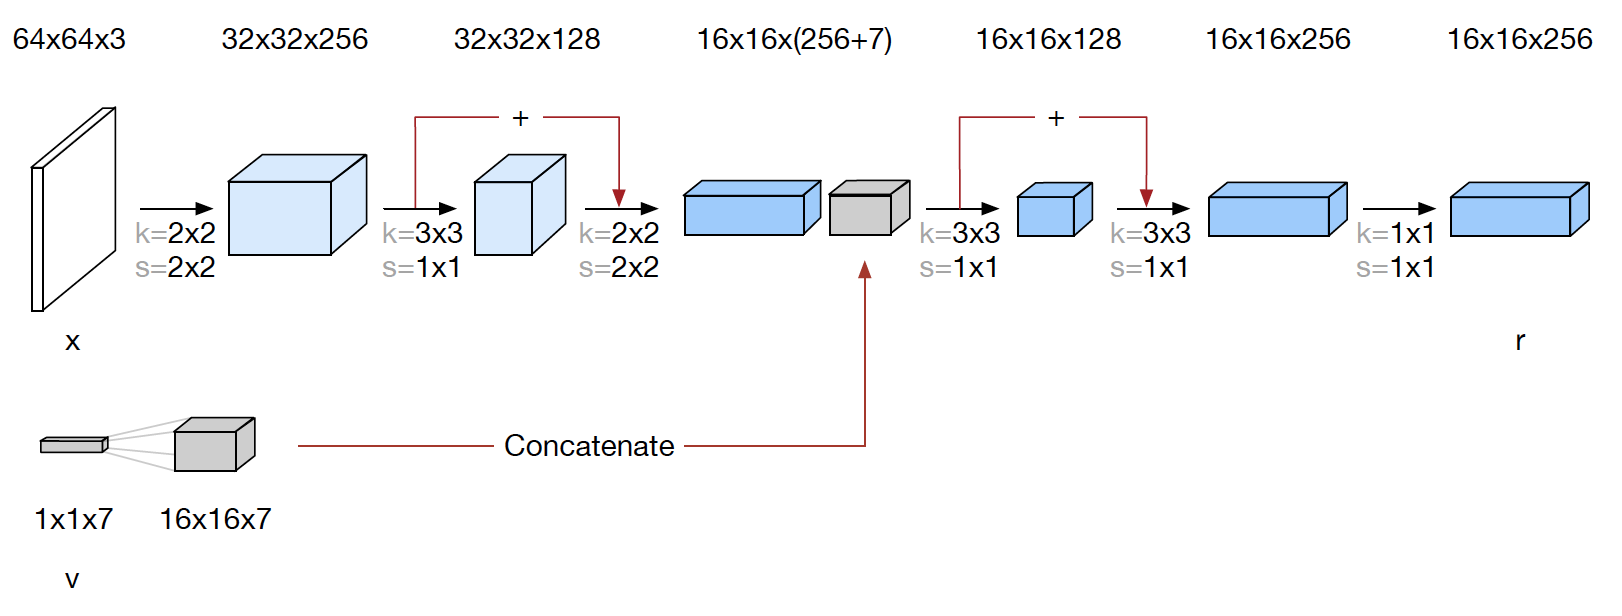
\includegraphics[width=\linewidth]{./figures/representation_network.png}
    \caption{推論ネットワークで用いるCNN(\cite{Eslami2018}より引用)}
    \label{fig:inference_network}
  \end{center}
\end{figure}

\subsection{生成ネットワーク}
生成ネットワークは,推論ネットワークを用いて得られた潜在変数$\bm{z} = {\{ \bm{z_l} \}}_{l=1}^L$とクエリである$\bm{v^ q}$からクエリに対応する観測$\bm{x^q}$を予測する.ここでもDRAWと同様に畳み込みLSTMと1層の畳み込みニューラルネットワークを用いてL回に分けて画像の生成を行う.具体的には,$\bm{v ^ q}$と$\bm{z_l}$を畳み込みLSTMの入力とし,その出力となる隠れ変数$\bm{h^g}$をさらに1層の畳み込みニューラルネットワークへの入力として,その出力を変数$\bm{u_l}$とする.これをL回繰り返し,最後に${\{ \bm{u_l} \}}_{l=1}^L$の要素ごとの和を入力とする畳み込みニューラルネットワークの出力を観測画像の予測$\bm{\hat{x}^q}$とする.

このようにして,生成ネットワークは画像の生成を行う.

\section{類似手法との差分の整理}
本節では,提案手法と類似手法の差分について,特に確率モデルの観点から整理する.提案手法と同様にFig. \ref{fig:gm_proposal}のような確率モデルを仮定し,それぞれのデータセットに固有の変数をコンテキストからamortized inferenceにより推論するニューラルネットワークを定義するメタ学習の手法として,Conditional Neural Processes(以下,CNPs)\cite{CNP}とNeural Processes(以下,NPs)\cite{NP}がある.

CNPsは,最適化に用いる目的関数は提案手法と同様であるが,生成クエリネットワークの場合と同様に,データセットに固有の変数$\bm{r_i}$を決定論的に推論しており,不確実性を考慮していない点が提案手法と大きく異なる.

% 一方で,NPsでは提案手法と同様に,データセットに固有の変数を確率的な変数$\bm{z_i}$とし,その不確実性を考慮しているが,学習時に新たな近似事後分布を用いて$\bm{z_i}$のサンプリングを行っている点が提案手法との差分である.このような近似事後分布を置くことは,学習の不安定性につながることは\ref{section:problem}で既に指摘した通りである.

ここまでの内容を整理すると,提案手法と生成クエリネットワーク,CNPs, NPsの関係はTable \ref{table:model_comparison}のようになる.

\begin{table}[tbp]
  \begin{center}
  \caption{提案手法と類似手法の比較}
  \scalebox{0.8}{
  \begin{tabular}{|c||c|c|c|} \hline
    手法 & データセット固有の変数への推論 & データ固有の変数 & 潜在変数の近似事後分布\\ \hline \hline
    生成クエリネットワーク & 決定論的 & あり & あり \\ \hline
    CNPs & 決定論的 & なし & なし \\ \hline
    NPs & 確率的 & なし & あり \\ \hline    
    提案手法 & 確率的 & なし & なし \\ \hline    
  \end{tabular}
  }
  \label{table:model_comparison}
  \end{center}
\end{table}

